\documentclass[]{article}

\usepackage{siunitx} % Provides the \SI{}{} and \si{} command for typesetting SI units
\usepackage{graphicx} % Required for the inclusion of images
\usepackage{amsmath} % Required for some math elements
\usepackage[letterpaper]{geometry} % 8.5 x 11 paper
\usepackage{listings}
\usepackage{hyperref}

%opening
\title{Linearity II\\Gradient Descent Homework}
\date{October 5, 2015}
\author{David Abrahams}

\begin{document}

\maketitle

\section{The contour plot}

I generated a contour plot for $f(x, y) = \sin(x)\sin(x + 3y)$ with the following python functions:

\begin{lstlisting}[language=Python, frame=single]
def function(x, y):
    return sin(x) * sin(x + 3 * y)

def contour(func, x_min, x_max, y_min, y_max):

    x = linspace(x_min, x_max)
    y = linspace(y_min, y_max)
    X, Y = meshgrid(x, y)

    Z = func(X, Y)

    CS = plt.contour(X, Y, Z)

def grad_f(x, y):
    d_dx = sin(2*x + 3*y)
    d_dy = 3 * sin(x) * cos(x + 3 * y)
    return d_dx, d_dy
\end{lstlisting}

\begin{figure}
\centering
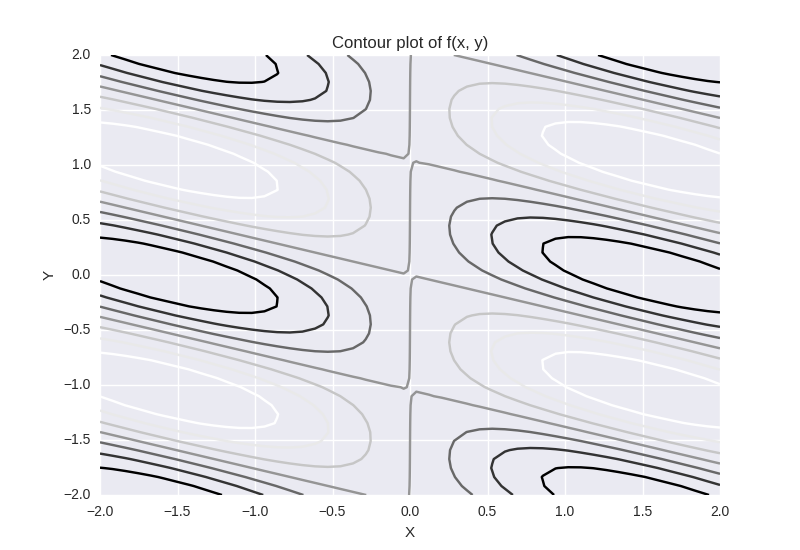
\includegraphics[height=3in]{../img/contour.png}
\caption{The contour plot}
\label{fig:contour}
\end{figure}

This produced the graph in Figure~\ref{fig:contour}. There are a series of hills and valleys where the $\sin$ functions peak and valley. Running the following code to show the \texttt{quiver}:

\begin{lstlisting}[language=Python, frame=single]]
def grad_f(x, y):
    d_dx = sin(2*x + 3*y)
    d_dy = 3 * sin(x) * cos(x + 3 * y)
    return d_dx, d_dy

def quiver(grad_func, x_min, x_max, y_min, y_max):
    x = linspace(x_min, x_max, num=20)
    y = linspace(y_min, y_max, num=20)
    X, Y = meshgrid(x, y)

    U, V = grad_func(X, Y)
    q = plt.quiver(X, Y, U, V)
\end{lstlisting}

produces Figure~\ref{fig:quiver}. The gradient points toward each of the hills, and away from the valleys.

\begin{figure}
\centering
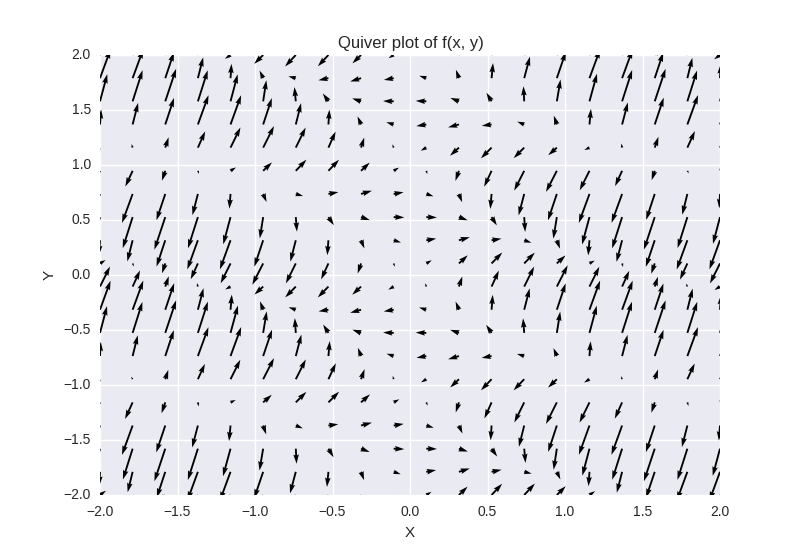
\includegraphics[height=3in]{../img/quiver.png}
\caption{The quiver plot}
\label{fig:quiver}
\end{figure}

To find a local maximum, I implemented a gradient descent algorithm. Starting from $(1, 1)$, it moves in the direction of the gradient.

\begin{lstlisting}[language=Python, frame=single]]
def descent(grad_func, x_0, y_0, lambda_val, n_iterations):

    res = vstack((array([x_0, y_0]), zeros((n_iterations, 2))))

    for i in range(1, n_iterations + 1):
        prev_x, prev_y = res[i - 1, :]
        gradient_x, gradient_y = grad_func(prev_x, prev_y)
        next_x = lambda_val * gradient_x + prev_x
        next_y = lambda_val * gradient_y + prev_y
        res[i, :] = [next_x, next_y]

    x = res[:, 0]
    y = res[:, 1]
    q = plt.quiver(x[:-1], y[:-1], x[1:]-x[:-1], y[1:]-y[:-1],
                   scale_units='xy', angles='xy', scale=1)
    return res
\end{lstlisting}

Using the parameters \texttt{lambda\_val=0.25, n\_iterations=10} produces the graph in Figure~\ref{fig:lambda25}. Using \texttt{lambda\_val=0.1} produces Figure~\ref{fig:lambda10}.

\begin{figure}
\centering
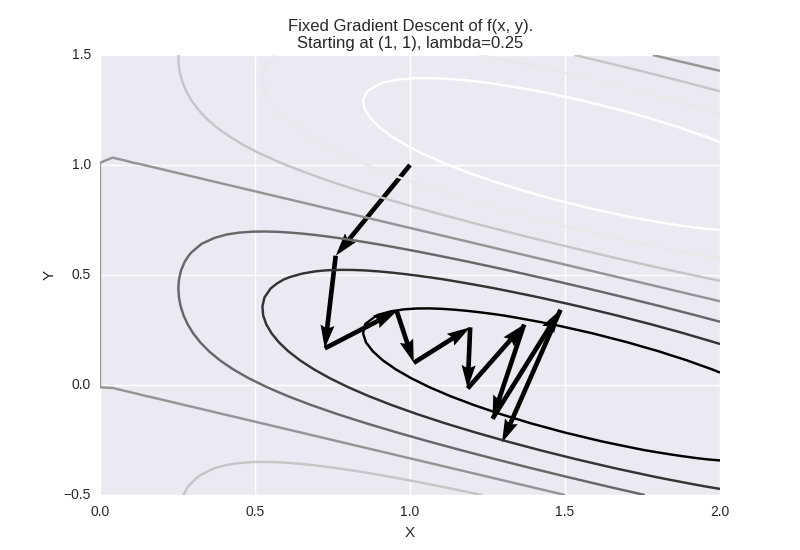
\includegraphics[height=3in]{../img/fixed_grad_25.png}
\caption{Gradient descent: \texttt{lambda\_val=0.25, n\_iterations=10}}
\label{fig:lambda25}
\end{figure}

\begin{figure}
\centering
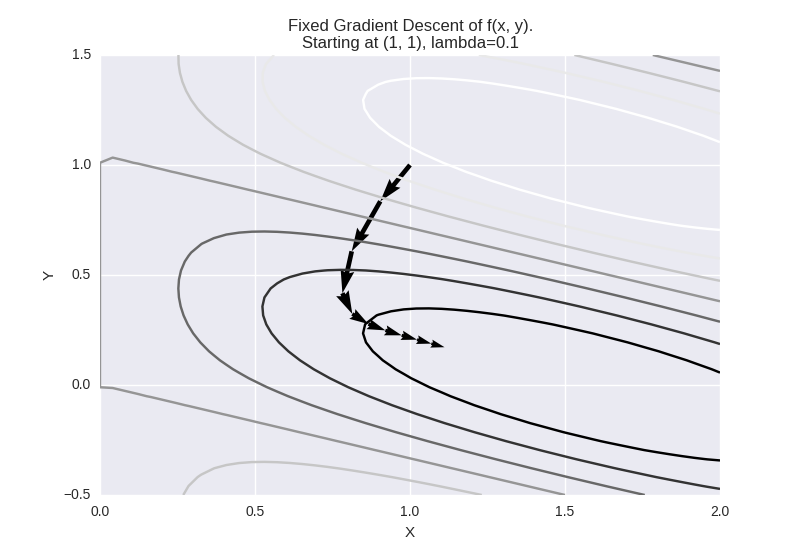
\includegraphics[height=3in]{../img/fixed_grad_10.png}
\caption{Gradient descent: \texttt{lambda\_val=0.1, n\_iterations=10}}
\label{fig:lambda10}
\end{figure}

Using \texttt{lambda\_val=0.25} fails to find the maximum because it bounces around it. \texttt{lambda\_val=0.10} moves too slowly. A better solution is to dynamically change lambda using \texttt{fmin} in order to reach the highest possible point at each step iteration.

\begin{lstlisting}[language=Python, frame=single]]
def accurate_descent(func, grad_func, x_0, y_0, n_iterations):

    res = vstack((array([x_0, y_0]), zeros((n_iterations, 2))))

    for i in range(1, n_iterations + 1):
        prev_x, prev_y = res[i - 1, :]
        gradient_x, gradient_y = grad_func(prev_x, prev_y)
        lambda_val = optimize_lambda(func, prev_x, prev_y, gradient_x,
                                     gradient_y)
        next_x = lambda_val * gradient_x + prev_x
        next_y = lambda_val * gradient_y + prev_y
        res[i, :] = [next_x, next_y]

    x = res[:, 0]
    y = res[:, 1]
    plt.quiver(x[:-1], y[:-1], x[1:]-x[:-1], y[1:]-y[:-1], scale_units='xy',
               angles='xy', scale=1)

    return res

def optimize_lambda(func, x_0, y_0, grad_x, grad_y):
    anon_func = lambda x: -f_x_lamba_f(func, x_0, y_0, grad_x, grad_y, x)
    return fmin(anon_func, 0)

def f_x_lamba_f(func, x_0, y_0, grad_x, grad_y, lambda_val):
    next_x = x_0 + grad_x * lambda_val
    next_y = y_0 + grad_y * lambda_val
    return func(next_x, next_y)
\end{lstlisting}

Doing $10$ iterations produces the graph in Figure~\ref{fig:lambdaopt}. This is clearly the most efficient algorithm, as it reaches the maximum relatively quickly.

\begin{figure}
\centering
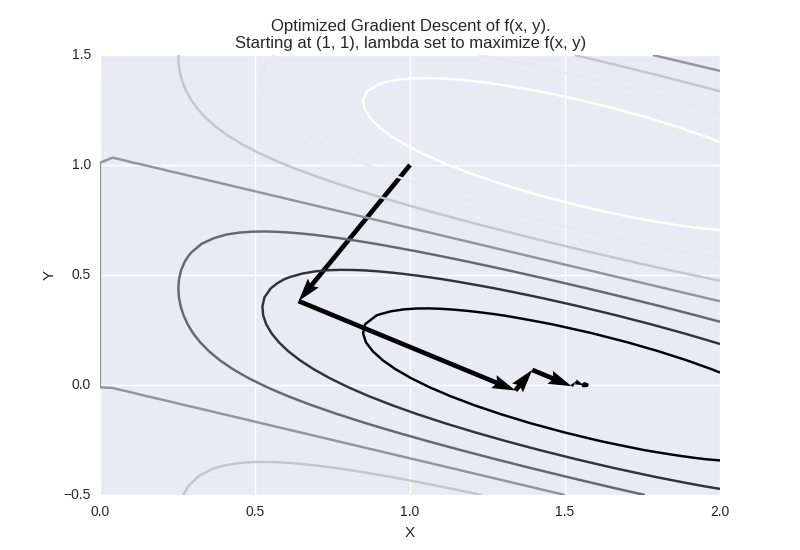
\includegraphics[height=3in]{../img/optimized_gradient.png}
\caption{Gradient descent, with \texttt{lambda} being set to the value that gets to the highest point at each step.}
\label{fig:lambdaopt}
\end{figure}

\end{document}
